As an ion is exposed to a laser, it continually excites and decays via spontaneous or stimulated emission. Given the laser detuning from resonance and intensity at the ion, the ion comes to an equilibrium where the fraction of time it occupies the excited and ground states is well defined. The integrated photon counts ($N$) from the iXon camera as a function of the laser intensity and detuning from resonance can be described by
\begin{align}
	N & = a \rho_{pp} \nonumber \\
	& = \frac{a}{2}\frac{s}{1+s+4(\delta/\Gamma)^2} \label{eq: fluor fit}
\end{align}
where $a$ contains the efficiency parameter $\epsilon$ from equation \ref{eq: fluorescence efficiency} as well as other unaccounted effects. By mapping the number of collected photons as a function of incident power and/or laser detuning allows us to fit equation \ref{eq: fluor fit} to find $a$. Although we may be able to determine $a$ once, we cannot guarantee that it stays the same from day to day as the total number of photons collected can change due to the temperature of the sensor, image focusing, etc. Once a fitted $a$ is found, we can then determine $\rho_{pp}$ as a function of laser power and detuning.

Having a single ion in the trap while sweeping the frequency or power would be ideal, but due to our loading process, we cannot reliably load only one ion, nor can we guarantee there only being one ion. On top of that, the most common residual gasses in a vacuum chamber, \ce{H2O} and \ce{H2} both readily react with \ce{Be+} in the excited state limiting the available interrogation time. Instead of a continuous measurement on one ion, we analyze images of ion chains at various laser powers and find the fluorescence per ion to fit to a generalized form of the scatter rate.

\ce{Be+} ions are loaded into the trap and A-ramps are applied until a chain is formed and the laser detuning adjusted until we see maximum fluorescence on the camera, which coincides with $\delta=\Gamma/2$. Images of the ions are taken at various laser powers and run through a maximum filter algorithm to identify the locations of individual \ce{Be+} ions as seen in Figure \ref{fig: ion image set}. The portion of the image determined not to be an ion is then averaged to obtain the background pixel value, which is then subtracted from each localized ion image. The pixel values over each localized ion is then summed to yield a total fluorescence value, which is then averaged for each image, as shown in Figure \ref{fig: local ions}. By performing a least squares fit on the collected fluorescence per ion as a function of incident power, we find the generalized efficiency $a$, revealing the P-state fraction at each power in $\rho_{pp}$, shown in Figure \ref{fig: p state curve}. This calibration can then be used to tune the P-state fraction using both laser power and frequency detuning.

\begin{figure}
	\centering
	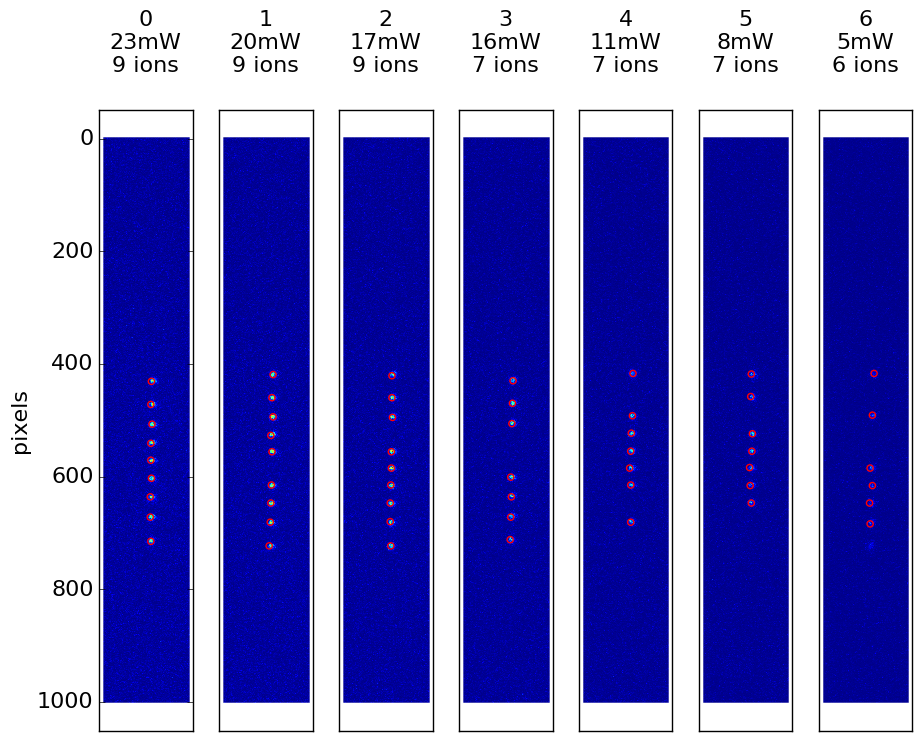
\includegraphics[width=0.8\textwidth]{images/ion_images.png}
	\caption{A set of ion images taken at various 313 nm powers run thorough a maximum filter algorithm that identifies local maxima, representing individual ions (circled in red). gaps in the ion chain are due to reactions with background \ce{H2} producing \ce{BeH+}, which occupy crystal sites without fluorescing.}
	\label{fig: ion image set}
\end{figure}

\begin{figure}[H]
	\centering
	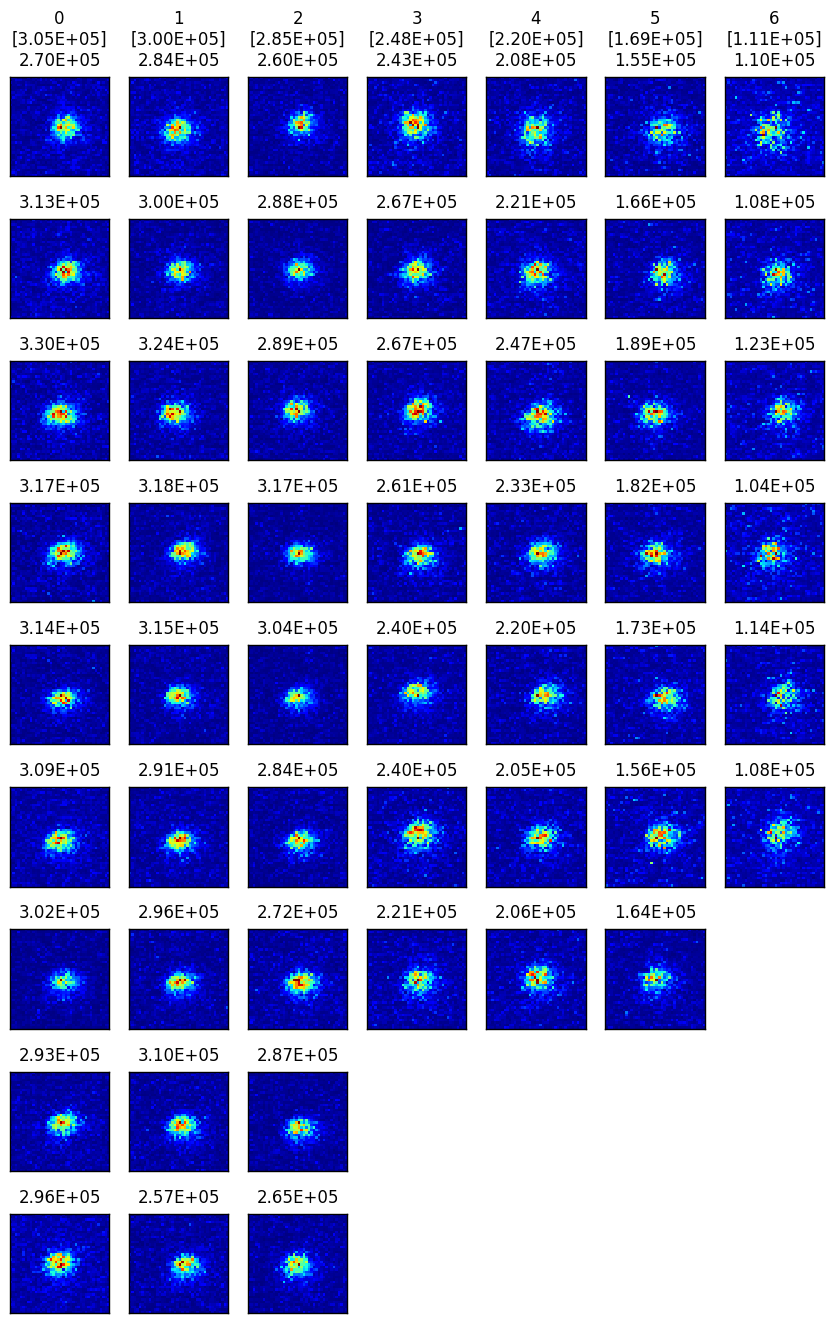
\includegraphics[height=0.7\paperheight]{images/isolated_ions.png}
	\caption{Individual ions identified from images in figure \ref{fig: ion image set}. Integrated pixel values with subtracted background counts shown for each image, a set's averaged value is shown in brackets.}
	\label{fig: local ions}
\end{figure}

\begin{figure}
	\centering
	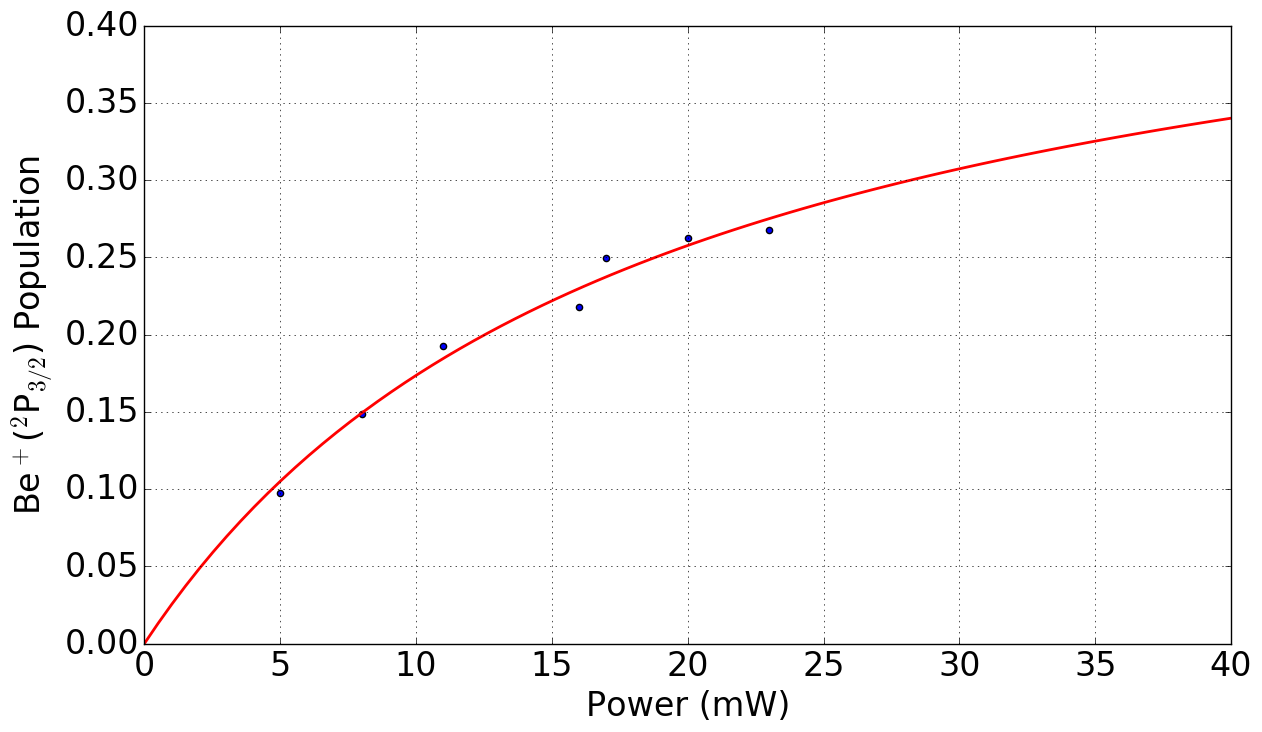
\includegraphics[width=0.8\textwidth]{images/P_state_curve.png}
	\caption{P-state fraction curve fitted to incident laser power at a fixed detuning of $\delta = \Gamma/2$. Total fluorescence value is normalized by fitted efficiency parameter $a$ to yield $\rho_{pp}$.}
	\label{fig: p state curve}
\end{figure}